\chapter{强监督分割方法及实现}
\section{引言}
强监督学习是相对于无监督学习、弱监督学习而言。尽管当前的技术已经取得了巨大的成功,但是值得注意的是,其方法非常依赖于大规模数据集的标注。该技术通过学习大量训练样本来构建预测模型,其中每个训练样本都有一个标签标明其真值输出。在图像分割领域,每个训练样本所对应的真值应该是像素语义级标注的,即对于图像中每一个像素所属的类别的信息都需要引入训练过程中。 而缺乏大型数据集使得最先进的强监督方法没有用武之地。本文的目的之一是提供一个大规模的白癜风数据集。希望本文的具有像素级标注的白癜风图像可以促进该视觉领域的研究。

本章首先介绍所提出的数据集,然后采用目前常用的强监督的方法对数据集进行测试。
\section{数据集:Vit2019}
现有的皮肤病图像数据集 \cite {mendoncca2013ph,codella2018skin,sun2016benchmark}包含有限的白癜风图像。为此,本文提出了一个新的临床白癜风数据集 “Vit2019”。据我所知,Vit2019是目前最大的像素级标注的白癜风图像数据集。简而言之,Vit2019包含两个类别的2,000个图像:1000个白癜风图像注释像素级和1000个非白癜风图像。样例见图\ref{fig:chap2_DatasetGragh1}。
\begin{figure}[htbp]
\begin{center}
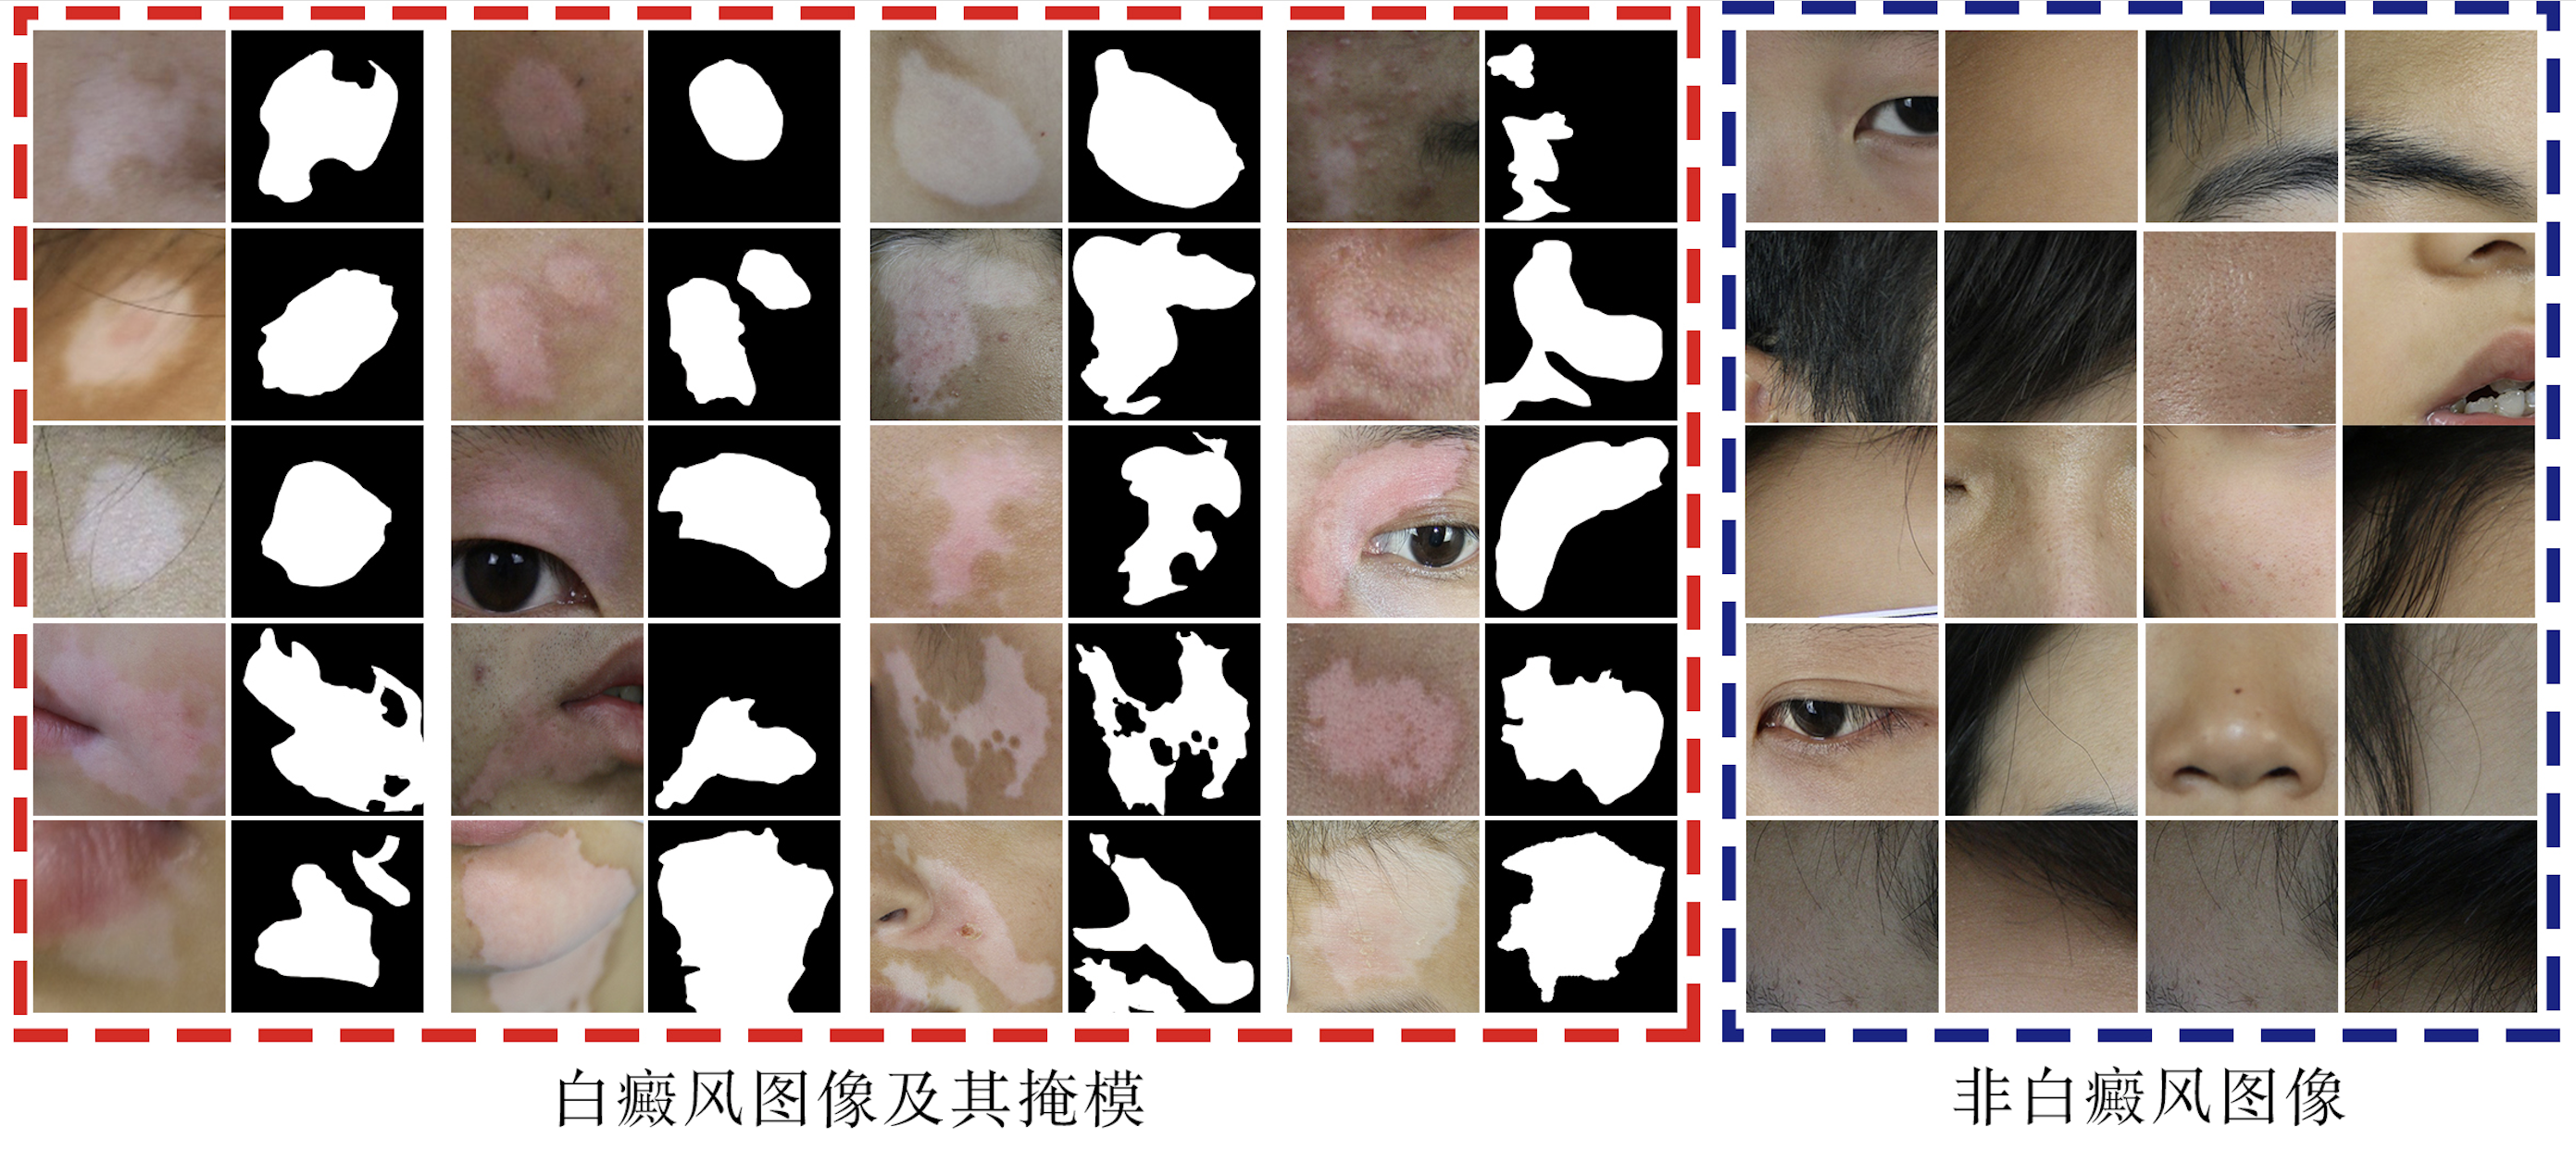
\includegraphics[width=\linewidth]{chap2_DatasetGragh1.png}
\end{center}
\caption{从Vit2019数据集中随机抽取的图像。 (a)白癜风图像。大约70%的图像位于患者的面部和颈部,而其余部分位于身体的其他部位(如躯干,胸部和背部)。 (b)非白癜风图像,其包含健康的皮肤,头发,眼睛,嘴唇,鼻子等。}
\label{fig:chap2_DatasetGragh1}
\end{figure}

\textbf{收集} ~大约800张图像由医院提供,其余图像则从互联网上收集(例如,谷歌图像,DERM101)。其他1,000张非白癜风图像是从没有白癜风病变的区域随机裁剪。

\textbf{标注}~像素级精确地注释白癜风区域是耗时且容易出错的。本文进行了像素级注释,并邀请了两位白癜风专家来审查此数据集,以确保注释质量。

\textbf {多样性}~ 此数据集是在现实世界条件下收集的。它涵盖了不同的环境因素,包括照明和摄像机视角,以及患者的其他属性,如年龄范围(儿童,青少年,老年人),皮肤状况(粗糙,光滑,健康,有其他色素性皮肤病),患病部位(面部,手部,脚部,四肢,头皮),性别,肤色(较深,较浅),不同阶段(早,中,晚)的病变,治疗程度(未经治疗,初始治疗后,经过长时间治疗)以及期限治疗。这使此数据集更加全面和具有挑战性。

\textbf {挑战}~由于数据集中大部分图像来源于临床,因此基于Vit2019中的分割任务在以下意义上具有挑战性:
\begin{enumerate}
\item Vit2019中的图像是在完全不受控制的情况下拍摄的,没有任何图像增强,例如去噪和对比度增强;
\item 图像主要以黄色皮肤为主,白癜风病变颜色浅(呈粉红色,浅黄色),对比度低,有些图像甚至需要专家来标记皮损的边界;
\item 如之前所述,受影响的区域是多样的。一些白癜风区域靠近眉毛或头皮,容易被头发阻挡,而唇部周围的一些白癜风区域易受唇部本身颜色的影响。
\end{enumerate}

\section{方法框架}

此处我们使用经典的``编码器解码器''的强监督分割框架Unet来对Vit2019上的图片进行训练和测试。具体的网络结构请参见第\ref{sec:fullySeg}节。

我们将Vit2019数据集的20\%作为测试集,另一部分作为训练集,在NVIDIA GTX-1080上进行训练,设置为 300个epochs,批量训练的大小设置为16张图片。开发语言选用Python, 深度学习框架使用Pytorch作为基础。Python编译器选用 Python 3.5.


\section{实验结果及分析}

\textbf{衡量指标}~
我们使用IoU这一评价指标来评价分割效果,如公式\ref{eq:IoU}所定义。IoU (Intersection over Union)是一种评估指标,用于衡量特定数据集上对象检测器或者分割的准确性。我们经常看到此评估指标用于图像分割方面的挑战,例如流行的MSCOCO挑战。为了应用Intersection over Union来评估分割效果,我们需要:分割的真值边界(即手工所标记边界,用于指定对象在我们图像中所占区域)和我们模型中预测的区域。我们利用这两组区域,就可以计算IoU。 
\begin{equation}
\label{eq:IoU}
\mathrm{IoU}=\frac{\mathrm {Area\,over\,Overlap}}{\mathrm {Area
\,of\,Union}}
\end{equation}
分子是我们预测的区域面积和真实的区域间的重叠区域。分母是两者区域的联合的区域。

\textbf{定性与定量结果}

如图\ref{fig:UnetResult}展示了U-net的分割效果,测试图片均为从测试集中随机抽取所得。第一列表示输入网络的原图,第二列表示U-net的分割结果,第三列表示手工标记的真值。我们可以发现,对于一些边界明显,对比度强的图片,U-net具有较好的分割能力,但是对于一些对比度差、边界模糊的图片,分割效果不尽如人意。而且可以观察到,U-net的分割结果对于边界细节的保持效果较差。

经过多组测试,得到平均的IoU为78.6\%.

\begin{figure}[htbp]
\begin{center}
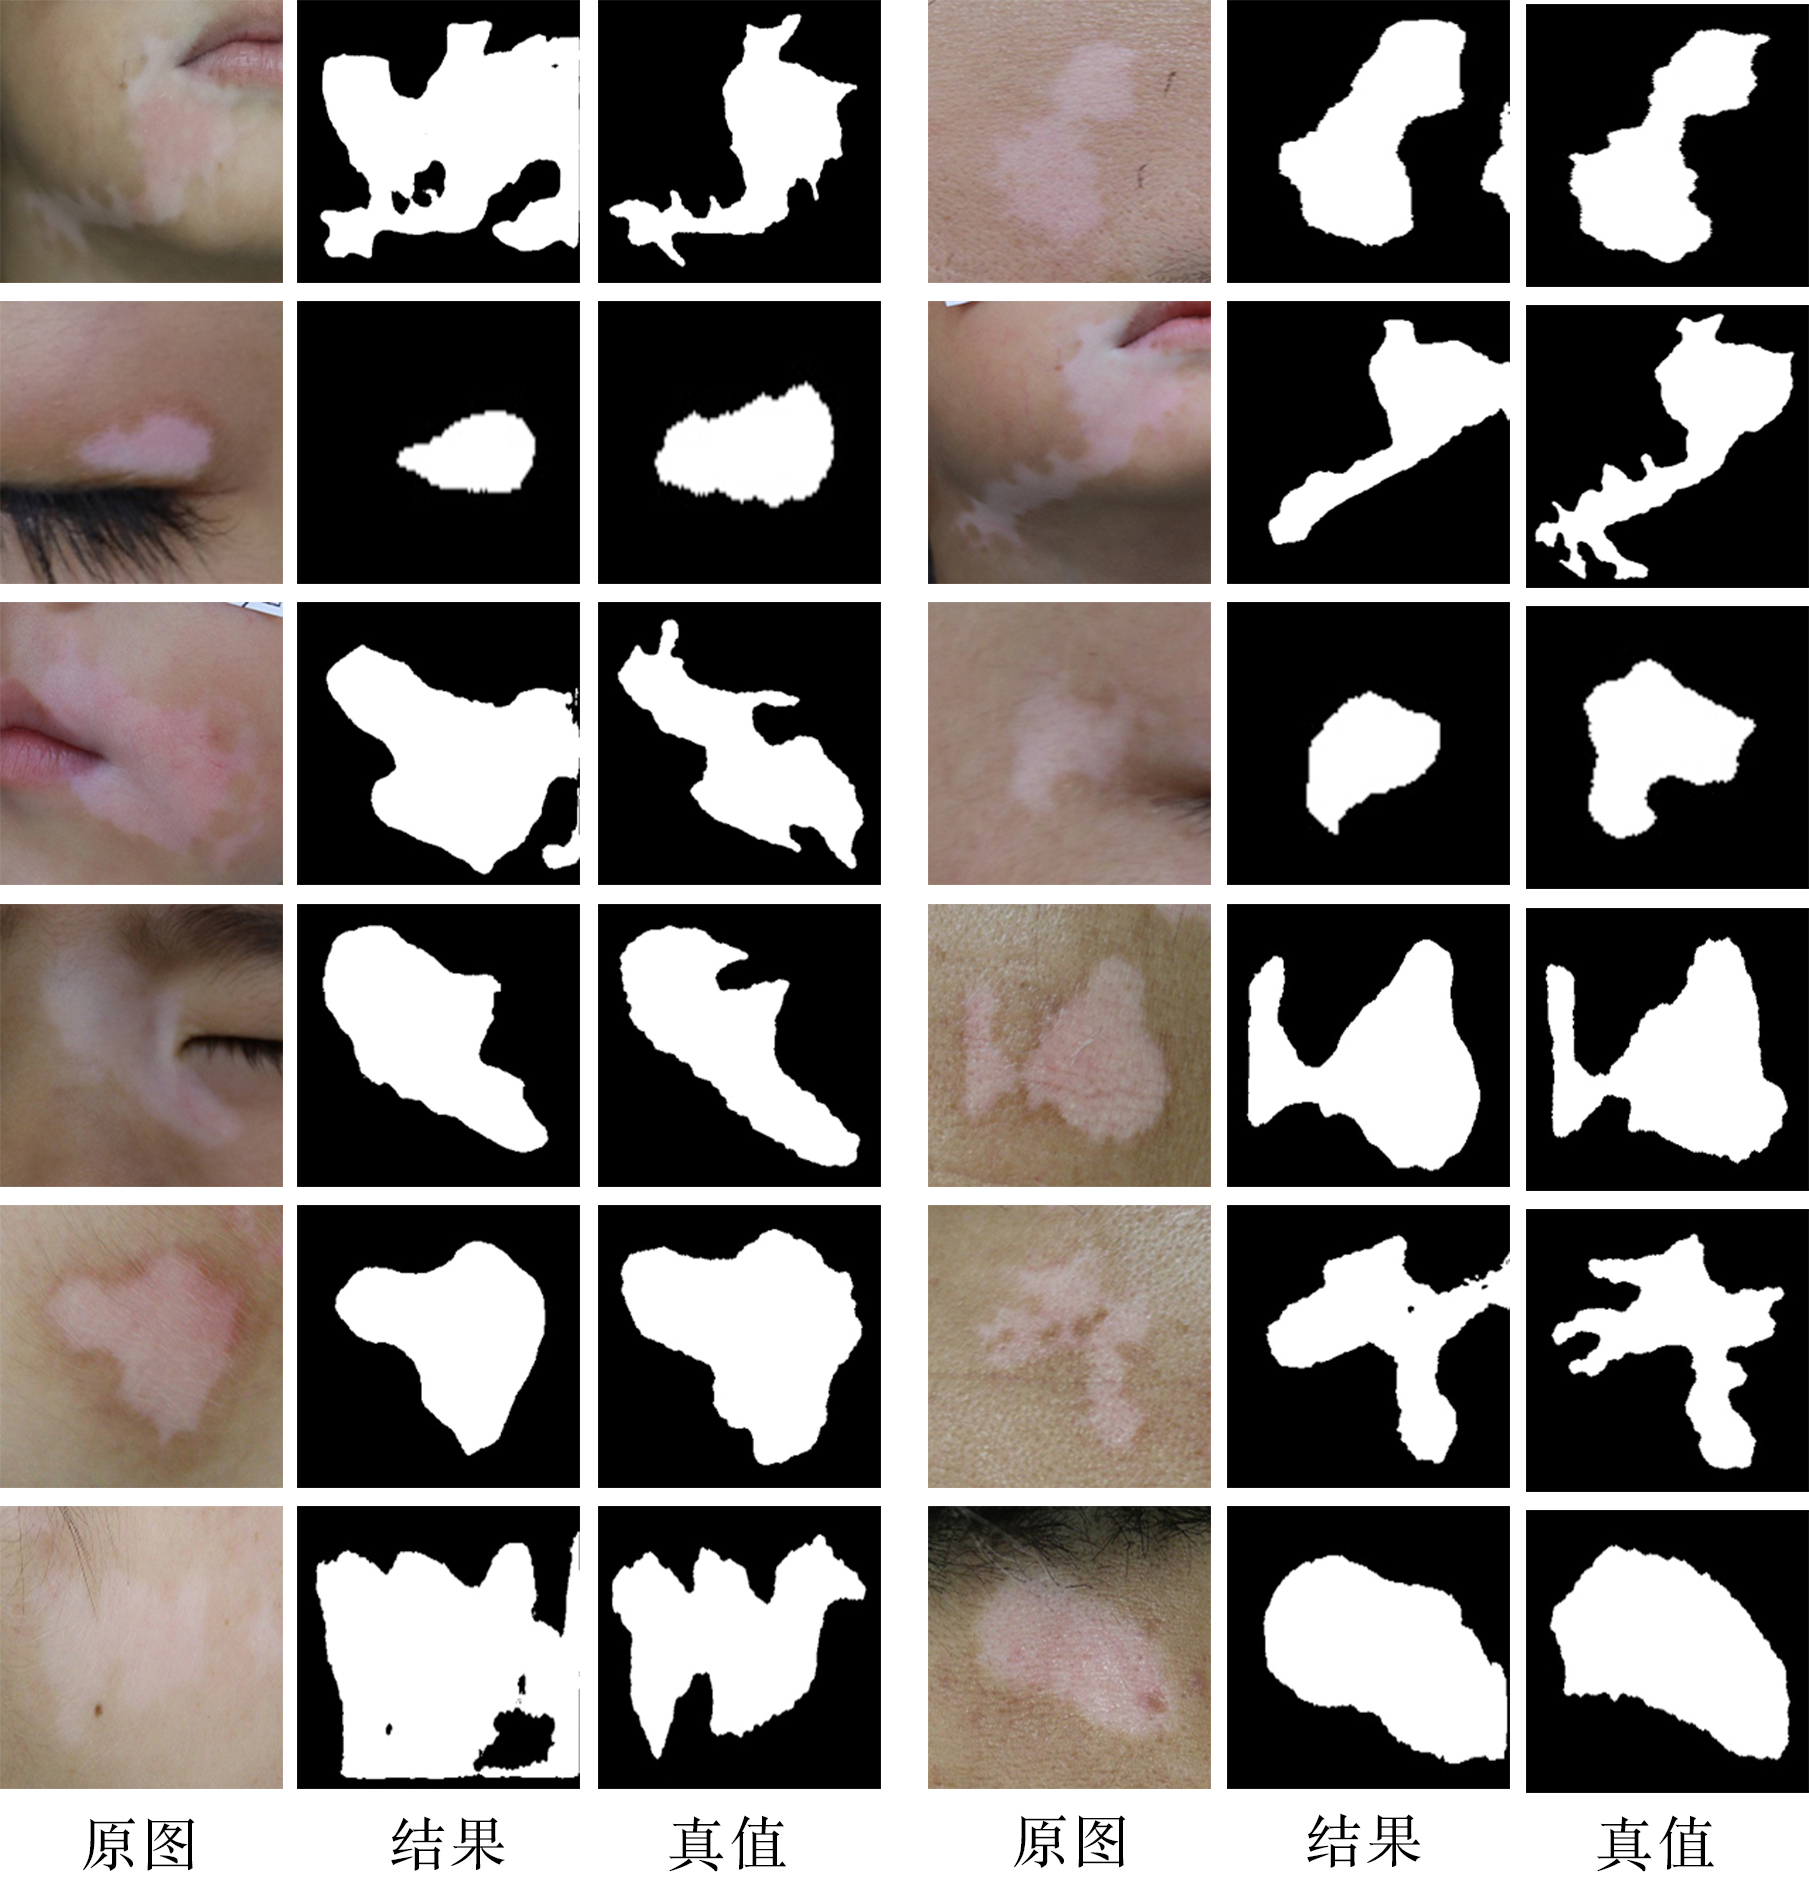
\includegraphics[width=0.7\linewidth]{UnetResult.jpg}
\end{center}
\vspace{-0.5cm}
\caption{Unet部分分割效果图}
\label{fig:UnetResult}
\end{figure}


\section{本章小结}
本章首先介绍了一些近些年来将深度学习应用于图像分割邻域的方法,然后引出了对于强监督学习而言,缺乏大规模的数据集会使得其没有用武之地的观点。于是紧接着介绍了本文所提出的数据集Vit2019,从收集、标注、多样性与挑战四个方面介绍了此数据集,并举例分析了一些样本图片。然后本文并着重介绍了一个经典的网络结构Unet,并且从定量和定性的角度展现并分析了Unet在Vit2019上的效果。在之后的弱监督学习的实验部分,本文也同样对比了强监督方法与现在最先进的弱监督方法的差距,用多项实验说明了本文所提出的弱监督分割方法可以很大程度的缩小与强监督方法之间的鸿沟。














